\documentclass{article}
\usepackage{fancyhdr} % 自定义页面的页眉和页脚样式
\usepackage{tocloft}  % 控制目录(包括目录、表格目录和插图目录)样式的命令
\usepackage{titlesec} % 自定义标题的样式,如章节标题、节标题等。
\usepackage{lipsum}   % 生成虚拟文本
\usepackage{biblatex} % 管理和生成参考文献列表
\usepackage{appendix} % 生成附录部分
\usepackage{listings} % 排版源代码块
\usepackage{geometry} % 设置页面布局
\usepackage{graphicx} % 插入图像并排列
\usepackage{subcaption} % 次级图像
\usepackage{amsmath}  %矩阵方能换行
\usepackage{times}    % 使用times new roman 字体
\usepackage{xeCJK}
\setCJKmonofont{仿宋}

% 设置目录格式
\renewcommand{\cfttoctitlefont}{\fontsize{15}{6}\normalfont}     % 将目录标题字体
\renewcommand{\cftsecfont}{\fontsize{15}{6}\normalfont}          % 设置章节标题字体
\renewcommand{\cftsubsecfont}{\fontsize{15}{6}\normalfont}       % 设置子节标题字体
\setlength{\cftbeforesecskip}{2em}               % 设置章节之间的垂直距离
\setlength{\cftbeforesubsecskip}{1em}          % 设置子节之间的垂直距离


% 设置页面布局
\geometry{
	left=3cm,
	right=3cm,
	top=3cm,
	bottom=2cm,
}

% 设置代码布局
\lstset{
	language=Python,
	numbers=left,
	frame=single,
	breaklines=true,
	breakatwhitespace=false,
	basicstyle=\small\ttfamily,
	showspaces=false, % 显示空格
}

% 设置页眉页脚
\pagestyle{fancy}
\fancyhf{}
\fancyhead[L]{蒙特卡洛方法}
\fancyhead[C]{李永阳}
\fancyhead[R]{\thepage}
\renewcommand{\headrulewidth}{0.4pt}

\titleformat{\section}{\fontsize{15}{6}\bfseries\itshape}{\thesection}{1em}{}
\titleformat{\subsection}{\fontsize{15}{6}\bfseries}{\thesubsection}{1em}{}

\begin{document}
	
	\thispagestyle{fancy}
	\pagenumbering{gobble} 
	\begin{center}
		\textbf{{\fontsize{15}{14}\itshape\selectfont
				蒙特卡洛方法\quad 作业1 }}
		\vspace{2em}
		
		\textbf{{\fontsize{15}{14}\itshape\selectfont
				\today{}
		}}
		\vspace{2em}
									
		\textbf{{\fontsize{15}{14}\itshape\selectfont 李永阳 2021141220025 }}
	\end{center}	
	
	\pagenumbering{arabic} % 正文页开始
	
	\section{}
	\subsection*{题1.3}
	\quad 
	
	我认为在此处使用$\delta$函数表示概率密度完全是多此一举,因此使用分布表表示:
	
	\begin{table}[ht]
	\centering
	\caption{概率分布表}
	\begin{tabular}{|c | c|c|c|}
		\hline
		$x$ & 0 & 1 & 2\\
		\hline
		$P$ & $\frac{1}{2}$ & $\frac{1}{3}$ & $\frac{1}{6}$ \\
		\hline
	\end{tabular}
	\end{table}
	
	显然有:
	
	\begin{equation*}
		\begin{split}
			&<x>=\sum P_i\cdot x_i\\
			&<x^2>=\sum P_i\cdot x_i^2\\
			&\sigma^2 = <x^2> - <x>^2
		\end{split}
	\end{equation*}

	因此我们可以得到:
	
	\begin{equation*}
		\begin{split}
			&<x>=\frac{2}{3}\\
			&<x^2>=1\\
			&\sigma^2=\frac{5}{9}\\
			&\sigma=\frac{\sqrt{5}}{3}
		\end{split}
	\end{equation*}
	
	我们给出CDF图像\ref{fig:1-3-CDF} 如下。
	
	
	\begin{figure}[!ht]
		\centering
		\caption{概率分布函数}
		\label{fig:CDF function}
		\begin{subfigure}[b]{0.4\textwidth}
			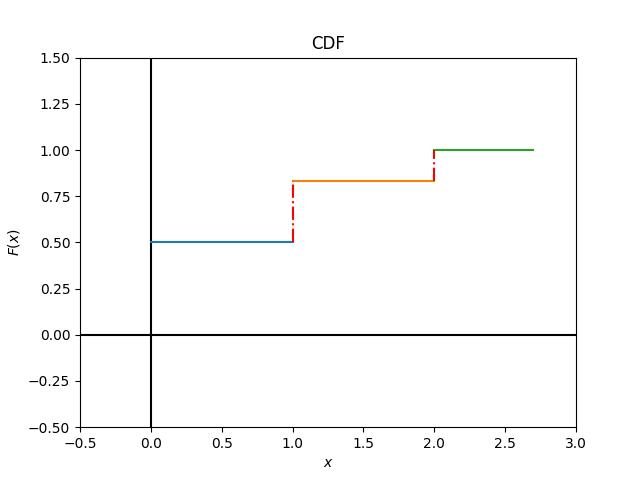
\includegraphics[width=\textwidth]{figure/1-3-CDF}
			\caption{题1.3 概率分布函数}
			\label{fig:1-3-CDF}
		\end{subfigure}
		\begin{subfigure}[b]{0.4\textwidth}
			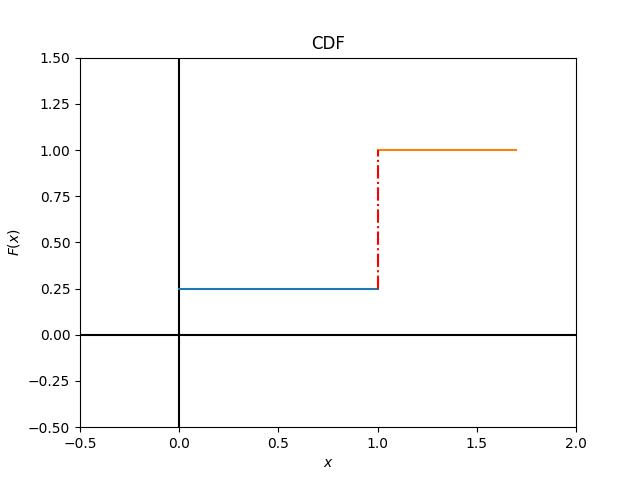
\includegraphics[width=\textwidth]{figure/1-2-CDF}
			\caption{题1.2 概率分布函数}
			\label{fig:1-2-CDF}
		\end{subfigure}
		\hfill
		\begin{subfigure}[b]{0.4\textwidth}
			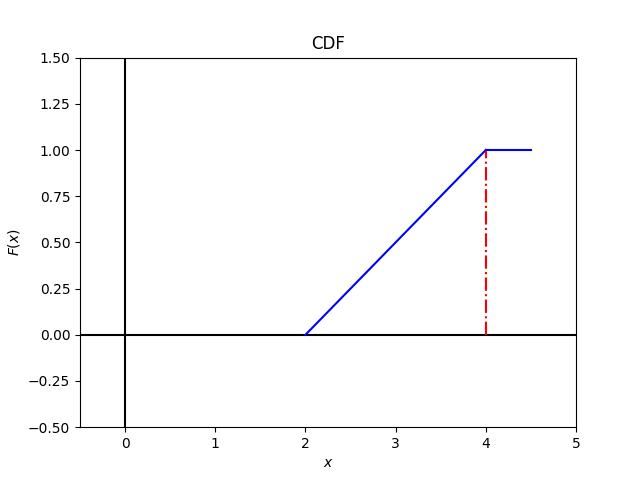
\includegraphics[width=\textwidth]{figure/1-5-CDF}
			\caption{题1.5 概率分布函数}
			\label{fig:1-5-CDF}
		\end{subfigure}
		\begin{subfigure}[b]{0.4\textwidth}
			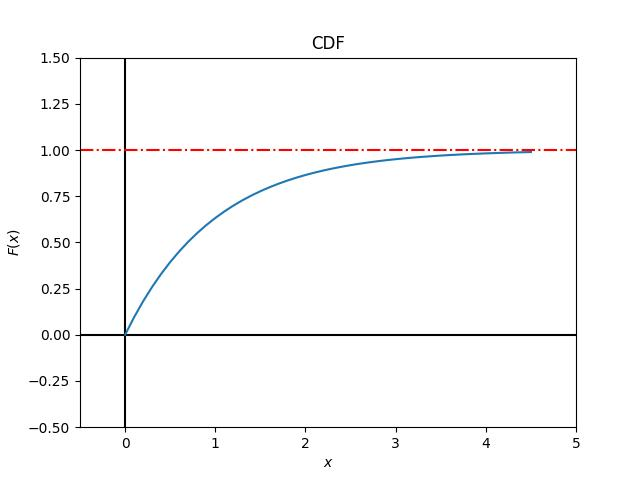
\includegraphics[width=\textwidth]{figure/1-6-CDF}
			\caption{题1.6 概率分布函数}
			\label{fig:1-6-CDF}
		\end{subfigure}		
	\end{figure}


	\subsection*{题1.2}
	\quad 
	
	同上题:
	
	\begin{table}[ht]
	\centering
	\caption{概率分布表}
	\begin{tabular}{|c|c|c|}
		\hline
		$x$ & 0 & 1\\
		\hline
		$P$ & $\frac{1}{4}$ & $\frac{3}{4}$  \\
		\hline
	\end{tabular}
	\end{table}	
	
	因此我们可以得到:

	\begin{equation*}
	\begin{split}
		&<x>=\frac{3}{4}\\
		&<x^2>=\frac{3}{4}\\
		&\sigma^2=\frac{3}{16}\\
		&\sigma=\frac{\sqrt{3}}{4}
	\end{split}
	\end{equation*}	
	
	我们给出CDF图像\ref{fig:1-2-CDF} 如下。
	
	\subsection*{题1.5}
	\begin{equation*}
		\begin{split}
			&<x>=\int_2^4 xf(x)dx = 3\\
			&<x^2>=\int_2^4 x^2f(x)dx = \frac{28}{3}\\
			&\sigma^2 = \frac{1}{3}\\
			&\sigma = \frac{\sqrt{3}}{3}
		\end{split}
	\end{equation*}
	
	我们给出CDF图像\ref{fig:1-5-CDF} 如上。
	
	我们给出PDF图像\ref{fig:1-5-PDF} 如下。


	\subsection*{题1.6}
	\begin{equation*}
		\begin{split}
			&<x>=\int_0^\infty xe^{-x}dx = 1\\
			&<x^2>=\int_0^\infty x^2e^{-x}dx = 2\\
			&\sigma^2 = 1\\
			&\sigma = 1
		\end{split}
	\end{equation*}

	我们给出CDF图像\ref{fig:1-6-CDF} 如上。
	
	我们给出PDF图像\ref{fig:1-6-PDF} 如下。
	
		
	\begin{figure}[!ht]
		\centering
		\caption{概率密度函数}
		\label{fig:CDF function}
		\begin{subfigure}[b]{0.4\textwidth}
			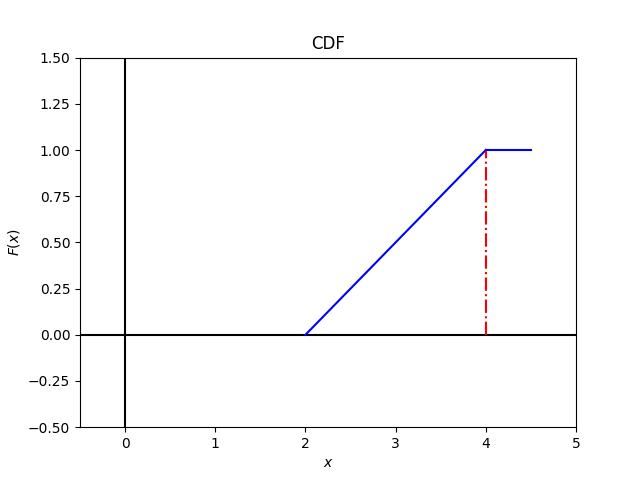
\includegraphics[width=\textwidth]{figure/1-5-CDF}
			\caption{题1.5 概率密度函数}
			\label{fig:1-5-PDF}
		\end{subfigure}
		%\hfill
		\begin{subfigure}[b]{0.4\textwidth}
			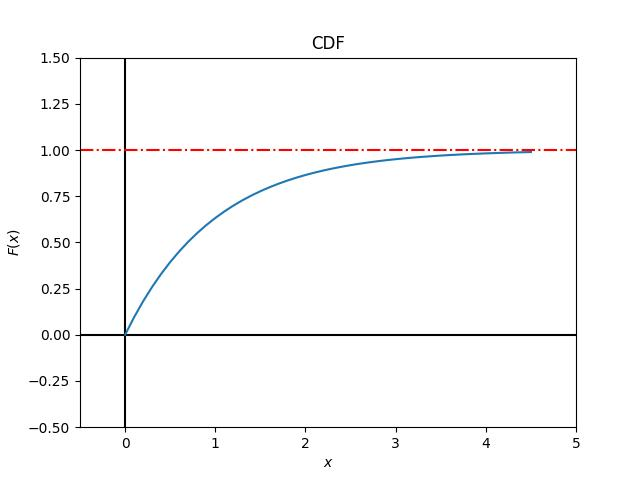
\includegraphics[width=\textwidth]{figure/1-6-CDF}
			\caption{题1.6 概率密度函数}
			\label{fig:1-6-PDF}
		\end{subfigure}
	\end{figure}
	
	\section{}
	\subsection*{题2.1}
	\quad 
	
	非常显然,有:
	\begin{equation*}
		y=\left\{
			\begin{split}
				0\quad\quad&x\in[0,0.5)\\
				1\quad\quad&x\in[0.5,5/6)\\
				2\quad\quad&x\in[5/6,1]
			\end{split}	
		\right.
	\end{equation*}
	
	\subsection*{题2.3}
	\quad 
	
	类似的,有
	\begin{equation*}
		\begin{split}
			z&=F(x)=\int_{-\infty}^x f(t)dt\\
			&=\int_{-h}^x\frac{dt}{2h}\\
			&=\frac{x+h}{2h}
		\end{split}
	\end{equation*}
	
	求出其反函数:$x=h(2z-1)$
	
	\subsection*{题2.6}
	\quad 
	
	同样的,有:
	\begin{equation*}
		\begin{split}
			z&=F(x)=\int_0^x f(t)dt\\
			&=\int_0^x 2te^{-t^2}dt\\
			&=1-e^{-x^2}
		\end{split}
	\end{equation*}
	
	求出其反函数:$x=\sqrt{-ln(1-z)}$
	
	\subsection*{题2.7}
	\quad 
	
	同样的,有:
	\begin{equation*}
		\begin{split}
			z&=F(x)=\int_0^x 3t^2dt\\
			&=x^3
		\end{split}
	\end{equation*}
	
	求出其反函数:$x=z^{1/3}$
	
	\section*{}
	\subsection*{2D-numerical-solution}
	\quad 
	
	显然该问题在二维情况下转换成利用蒙特卡洛方法计算积分
	\begin{equation*}
		\int_0^2\int_0^2 3-\frac{x}{2} - \frac{y}{2}dxdy
	\end{equation*}
	
	我们利用numpy1.25.1 中自带的0-1随机数生成器numpy.random.random计算程序,numpy版本号可以利用指令$numpy.\_\_version\_\_$查询
	
	取样点数:$1e7$
	
	计算结果:$8.000621379470351 \pm 0.00012908204728442695$
	
	计算精度:$1e-3$
	
	\subsection*{3D-numerical-solution}
	\quad 
	
	我不是很理解题中在$3D$绘景下计算具体指的是什么意思,不过我猜测是在$[0,2]\times[0,2]\times[0,3]$中随机撒点,通过统计在题中所说平面之下的点的数目来估计体积。依然利用numpy1.25.1 中自带的0-1随机数生成器numpy.random.random计算程序。
	
	取样点数:$1e7$
	
	计算结果:$8.001054 \pm 0.0017887365957195208$
	
	计算精度:$1e-2$
	
	\section*{十维蒙特卡洛积分}
	\quad 
	
	我们当然的意识到,十维蒙特卡洛积分与二维蒙特卡洛积分并无太大区别。我们还可以猜想到,随着蒙特卡洛积分维度的增加,其精度的增加速度必然是在下降的。
	
	取样点数为:$1e6$

	计算结果:$0.28884213742394654 \pm 3.0800365850647203e-06$

	计算精度:$1e-2$	
	
	取样点数为:$1e7$
	
	计算结果:$0.28430519116979497 \pm 9.449811116292106e-07$
	
	计算精度:$1e-2$
	
	取样点数为:$1e8$

	计算结果:$0.2847903425129942 \pm 3.0051152344585305e-07$

	计算精度:$1e-2$	
	
	
	\begin{thebibliography}{9}
		此次homework未用到任何参考文献
	\end{thebibliography}
	
	% 附录页
	\newpage 
	\appendix % 标记后续部分为附录
	\section*{Appendix}
	这是此次homework用到的全部代码
	
	图像绘制代码:
	\begin{lstlisting}
import os
figure_save_path = "figure"
import warnings
warnings.filterwarnings("error")
import numpy as np
np.random.seed(0)
import matplotlib.pyplot as plt
from PIL import Image


##plt.title("CDF")
##plt.xlabel("$x$")
##plt.ylabel("$F(x)$", rotation=90)
##plt.xlim(-0.5, 2)
##plt.ylim(-0.5, 1.5)
##plt.axhline(0, c="black")
##plt.axvline(0, c="black")
##x1 = np.arange(0, 1.1, 0.1)
##x2 = np.arange(1, 1.8, 0.1)
##plt.plot(x1, 1/4*np.ones(x1.size))
##plt.plot(x2, 1*np.ones(x2.size))
##plt.plot([1, 1], [1/4, 1], "r-.")
##if not os.path.exists(figure_save_path):
##    os.makedirs(figure_save_path)
##plt.savefig(os.path.join(figure_save_path, "1-2-CDF" + ".jpg"))

##plt.title("CDF")
##plt.xlabel("$x$")
##plt.ylabel("$F(x)$", rotation=90)
##plt.xlim(-0.5, 3)
##plt.ylim(-0.5, 1.5)
##plt.axhline(0, c="black")
##plt.axvline(0, c="black")
##x1 = np.arange(0.0, 1.1, 0.1)
##x2 = np.arange(1.0, 2.1, 0.1)
##x3 = np.arange(2.0, 2.8, 0.1)
##plt.plot(x1, 1/2*np.ones(x1.size))
##plt.plot(x2, 5/6*np.ones(x2.size))
##plt.plot(x3, 1*np.ones(x3.size))
##plt.plot([1, 1], [1/2, 5/6], "r-.")
##plt.plot([2, 2], [5/6, 1], "r-.")
##if not os.path.exists(figure_save_path):
##    os.makedirs(figure_save_path)
##plt.savefig(os.path.join(figure_save_path, "1-3-CDF" + ".jpg"))

##plt.title("PDF")
##plt.xlabel("$x$")
##plt.ylabel("$P(x)$")
##plt.xlim(1.5, 4.5)
##plt.ylim(0.0, 0.8)
##plt.axhline(0, c="black")
##plt.axvline(0, c="black")
##x1 = np.arange(2, 4.1, 0.1)
##plt.plot(x1, 1/2*np.ones(x1.size))
##plt.plot([2, 2], [0, 0.5], "r-.")
##plt.plot([4, 4], [0, 0.5], "r-.")
##if not os.path.exists(figure_save_path):
##    os.makedirs(figure_save_path)
##plt.savefig(os.path.join(figure_save_path, "1-5-PDF" + ".jpg"))

##plt.title("CDF")
##plt.xlabel("$x$")
##plt.ylabel("$F(x)$")
##plt.xlim(-0.5, 5.0)
##plt.ylim(-0.5, 1.5)
##plt.axhline(0, c="black")
##plt.axvline(0, c="black")
##x1 = np.arange(2, 4.1, 0.1)
##f = lambda x:0.5*(x-2)
##plt.plot(x1, f(x1), c="b")
##plt.plot([4, 4], [0, 1], "r-.")
##plt.plot([4, 4.5], [1, 1], c="b")
##if not os.path.exists(figure_save_path):
##    os.makedirs(figure_save_path)
##plt.savefig(os.path.join(figure_save_path, "1-5-CDF" + ".jpg"))

##plt.title("CDF")
##plt.xlabel("$x$")
##plt.ylabel("$F(x)$")
##plt.xlim(-0.5, 5.0)
##plt.ylim(-0.5, 1.5)
##plt.axhline(0, c="black")
##plt.axvline(0, c="black")
##x1 = np.arange(0, 4.6, 0.1)
##f = lambda x:1-np.exp(-x)
##plt.plot(x1, f(x1))
##plt.axhline(1, c="r", linestyle="-.")
##if not os.path.exists(figure_save_path):
##    os.makedirs(figure_save_path)
##plt.savefig(os.path.join(figure_save_path, "1-6-CDF" + ".jpg"))

plt.title("PDF")
plt.xlabel("$x$")
plt.ylabel("$P(x)$")
plt.xlim(-0.5, 4.5)
plt.ylim(-0.2, 1.2)
plt.axhline(0, c="black")
plt.axvline(0, c="black")
f = lambda x:np.exp(-x)
x1 = np.arange(0, 4.1, 0.1)
plt.plot(x1, f(x1))
if not os.path.exists(figure_save_path):
os.makedirs(figure_save_path)
plt.savefig(os.path.join(figure_save_path, "1-6-PDF" + ".jpg"))

	\end{lstlisting}

	题五代码一:蒙特卡洛方法二维积分

	\begin{lstlisting}	
import os
figure_save_path = "file_fig"
import warnings
warnings.filterwarnings("error")
import numpy as np
np.random.seed(0)
import matplotlib.pyplot as plt
from PIL import Image

print("RNG:", "Python numpy.random.random")

X_start = 0
Y_start = 0

X_end = 2
Y_end = 2

N = 10000000

num_points     = list(range(N))
random_xpoints = np.random.uniform(X_start, X_end, N)
random_ypoints = np.random.uniform(Y_start, Y_end, N)

X = np.arange(X_start, X_end, 100)
Y = np.arange(Y_start, Y_end, 100)

f = lambda i: 3 - random_xpoints[i]/2 - random_ypoints[i]/2
guess = np.array(list(map(f, num_points)))
ave = sum(guess)/N
I = ave*(X_end-X_start)*(Y_end-Y_start)

S2 = sum((guess-ave)**2)/(N-1)
S  = S2**0.5

print(I, "\pm", S/N**0.5)

##running result
##RNG: Python numpy.random.random
##8.000621379470351 \pm 0.00012908204728442695
		
	\end{lstlisting}

	题五代码二:蒙特卡洛方法二维点估计

\begin{lstlisting}	
import os
figure_save_path = "file_fig"
import warnings
warnings.filterwarnings("error")
import numpy as np
np.random.seed(0)
import matplotlib.pyplot as plt
from PIL import Image

print("RNG:", "Python numpy.random.random")
N = 10000000

num            = list(range(N))
xpoints = np.random.random(N) * 2
ypoints = np.random.random(N) * 2
zpoints = np.random.random(N) * 3

V = 2 * 2 * 3

f = lambda i:zpoints[i]<=3-xpoints[i]/2-ypoints[i]/2

counts = np.sum(np.array(list(map(f, num))))
ave = counts/N
S2  = counts*(1-ave)**2/(N-1) + (N-counts)*ave**2/(N-1)
S   = S2**0.5
print(ave*V, "\pm", S/N**0.5*V)

\end{lstlisting}
	
	题七代码:
\begin{lstlisting}
import os
figure_save_path = "figure"
import warnings
warnings.filterwarnings("error")
import numpy as np
np.random.seed(0)
import matplotlib.pyplot as plt
from PIL import Image

X1_start = 0
X2_start = 0
X3_start = 0
X4_start = 0
X5_start = 0

X6_start = 0
X7_start = 0
X8_start = 0
X9_start = 0
X0_start = 0


X1_end = 2
X2_end = 2
X3_end = 2
X4_end = 2
X5_end = 2

X6_end = 2
X7_end = 2
X8_end = 2
X9_end = 2
X0_end = 2


N = 100000000

num_points     = list(range(N))
random_x1points = np.random.uniform(X1_start, X1_end, N)
random_x2points = np.random.uniform(X2_start, X2_end, N)
random_x3points = np.random.uniform(X3_start, X3_end, N)
random_x4points = np.random.uniform(X4_start, X4_end, N)
random_x5points = np.random.uniform(X5_start, X5_end, N)

random_x6points = np.random.uniform(X6_start, X6_end, N)
random_x7points = np.random.uniform(X7_start, X7_end, N)
random_x8points = np.random.uniform(X8_start, X8_end, N)
random_x9points = np.random.uniform(X9_start, X9_end, N)
random_x0points = np.random.uniform(X0_start, X0_end, N)

f = lambda i: np.exp(-(random_x1points[i]**2 +
random_x2points[i]**2 +
random_x3points[i]**2 +
random_x4points[i]**2 +
random_x5points[i]**2 +

random_x6points[i]**2 +
random_x7points[i]**2 +
random_x8points[i]**2 +
random_x9points[i]**2 +
random_x0points[i]**2 ))

guess = np.array(list(map(f, num_points)))
ave = sum(guess)/N
I = ave*(X1_end-X1_start)*\
(X2_end-X2_start)*\
(X3_end-X3_start)*\
(X4_end-X4_start)*\
(X5_end-X5_start)*\
(X6_end-X6_start)*\
(X7_end-X7_start)*\
(X8_end-X8_start)*\
(X9_end-X9_start)*\
(X0_end-X0_start)

S2 = sum((guess-ave)**2)/(N-1)
S  = S2**0.5

print(I, "\pm", S/N**0.5)
	
\end{lstlisting}
	
\end{document}
